% Created 2016-08-17 Wed 14:38
\documentclass[tikz]{standalone}

\usepackage[utf8]{inputenc}
\usepackage[T1]{fontenc}

\usepackage{circledsteps}

\RequirePackage{xcolor}

%% HPI color definitions according to the design manual
% These do not exactly match the RGB values used in the Powerpoint slide master due to unknown reasons
\definecolor{hpiyellow}{RGB}{246,168,0}
\definecolor{hpiorange}{RGB}{221,97,8}
\definecolor{hpired}{RGB}{177,6,58}
\definecolor{hpigray}{RGB}{90,96,101}
\definecolor{hpiblue}{RGB}{0,122,158}


\renewcommand{\sfdefault}{neosans}
% Different font weights for neosans
\newcommand{\textl}[1]{{\fontseries{l}\selectfont #1}} % light
\newcommand{\textm}[1]{{\fontseries{m}\selectfont #1}} % medium, same as default weight
\newcommand{\textsb}[1]{{\fontseries{sb}\selectfont #1}} % semibold
\newcommand{\textmb}[1]{{\fontseries{mb}\selectfont #1}} % bold, same as \textbf
\newcommand{\texteb}[1]{{\fontseries{eb}\selectfont #1}} % extra bold
\newcommand{\textub}[1]{{\fontseries{ub}\selectfont #1}} % ultra bold

\tikzset{every picture/.style={/utils/exec={\sffamily}}}
\tikzset{flipflop RSflanke/.style={
  flipflop,
  flipflop def={t1=S, t2=C, c2=1, t3=R, t6=Q, t4={\ctikztextnot{Q}}}
}}


\tikzset{
  mechanicalSwitch/.pic={
    \coordinate (-inUp) at (135:2); 
    \coordinate (-inDown) at (235:2);
    \coordinate (-out) at (2,0);
    \coordinate (-center) at (0,0);
    
    \draw (0,0) circle [radius = 2cm];
    \draw [fill=gray!20] (0,0) circle [radius = 0.2cm];

    \draw (0, 0) -- (2, 0);
    \draw (135:.8) -- (135:2); 
    \draw (225:.8) -- (225:2); 

    \draw [fill=gray!20] (2, 0) circle [radius=0.05cm]; 
    \draw [fill=gray!20] (135:2) circle [radius=0.05cm]; 
    \draw [fill=gray!20] (225:2) circle [radius=0.05cm]; 

    
    \draw [thick] (0,0) -- (175:1.5); 

    \draw [dashed, <->, domain=135:225] plot ({cos(\x)}, {sin(\x)}); 
  },
  mechanicalSwitchClosed/.pic={
    \coordinate (-inUp) at (135:2); 
    \coordinate (-inDown) at (255:2);
    \coordinate (-out) at (2,0);
    \coordinate (-center) at (0,0);
    \draw (0,0) circle [radius = 2cm];
    \draw [fill=gray!20] (0,0) circle [radius = 0.2cm];

    \draw (0, 0) -- (2, 0);
    \draw (135:.8) -- (135:2); 
    \draw (225:.8) -- (225:2); 

    \draw [fill=gray!20] (2, 0) circle [radius=0.05cm]; 
    \draw [fill=gray!20] (135:2) circle [radius=0.05cm]; 
    \draw [fill=gray!20] (225:2) circle [radius=0.05cm]; 

    
    \draw [thick] (0,0) -- (135:2); 

    \draw [dashed, <->, domain=135:225] plot ({cos(\x)}, {sin(\x)}); 
  }
}


\usetikzlibrary{calc}
\usetikzlibrary{positioning}


\usepackage{../../templates/moeptikz}

\usetikzlibrary{chains}

\tikzset{
  % TODO: turn this into a proper TIKZ node for proper anchoring 
  pics/queue/.style args={#1 scale #2}{
    code={
      \begin{scope}[scale=#2]        
      \foreach \i in {1,...,#1} {
        \path [pic actions] (\i-1,0) rectangle (\i,1);
      }
      \path [draw] (-1.5,0) -- (0,0) (0,1) -- (-1.5,1);
      \path [draw, ->] (-2,0.5) -- (-1,0.5);
      \end{scope}
      
    }
  }
}

\begin{document}


\begin{tikzpicture}
  \label{page:cc:basic_scenario}
  \node [client] (client1) {};
  
  \node [switch,below right=of client1] (r1) {};
  \node [switch,right=of r1] (r2) {};

  \node [server, right=of r2] (s) {};

  \node [client, below left=of r1] (client2) {};

  \draw (r1) edge[thick] node[above right] {10 Gbps} (client1)
  edge [very thick] node[below right] {40 Gbps} (client2)
  to [thin] node[above] {1 Gbps} (r2)
  edge [very thick] node [above] {100 Gbps} (s)
  ; 
\end{tikzpicture}

\begin{tikzpicture}
  \label{page:cc:basic_scenario:with_queues}

  \node [client] (client1) {};
  
  \node [switch,below right=of client1] (r1) {};
  \node [switch,right=of r1] (r2) {};

  \node [server, right=of r2] (s) {};

  \node [client, below left=of r1] (client2) {};

  \draw (r1) edge[thick] node[above right] {10 Gbps} (client1)
  edge [very thick] node[below right] {40 Gbps} (client2)
  to [thin] node[above] {1 Gbps} (r2)
  edge [very thick] node [above] {100 Gbps} (s)
  ;

  \pic [draw, fill=hpired!30, rotate=0] at ($(r1.east)+(-1, -0.1)$) {queue={4 scale 0.25}}; 

  \pic [draw, fill=hpiblue!30, rotate=180] at ($(r2.west)+(1.4, 0.1)$) {queue={5 scale 0.25}}; 
  
\end{tikzpicture}


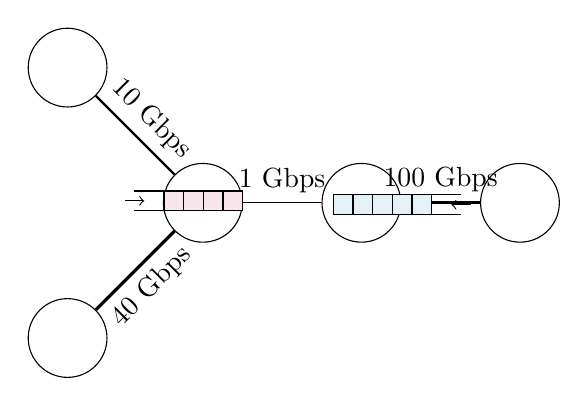
\begin{tikzpicture}
    
  \label{page:cc:just_test}
  \node [circle, minimum width=1cm, draw] (client1) {};
  
  \node [circle, minimum width=1cm, draw,below right=of client1] (r1) {};
  \node [circle, minimum width=1cm, draw,right=of r1] (r2) {};

  \node [circle, minimum width=1cm, draw, right=of r2] (s) {};

  \node [circle, minimum width=1cm, draw, below left=of r1] (client2) {};

  \draw (r1) edge[thick] node[above, sloped] {10 Gbps} (client1)
  edge [very thick] node[below, sloped] {40 Gbps} (client2)
  to [thin] node[above] {1 Gbps} (r2)
  edge [very thick] node [above] {100 Gbps} (s)
  ; 

  \pic [draw, fill=hpired!10, rotate=0] at ($(r1.east)+(-1, -0.1)$) {queue={4 scale 0.25}}; 

  \pic [draw, fill=hpiblue!10, rotate=180] at ($(r2.west)+(1.4, 0.1)$) {queue={5 scale 0.25}}; 
  
\end{tikzpicture}

%----------------------------------------------
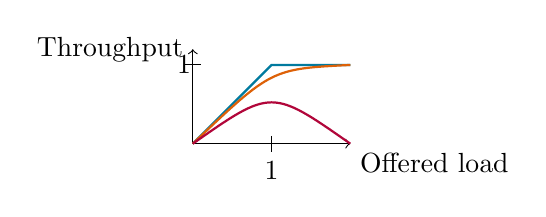
\begin{tikzpicture}
  \label{page:cc:ideal_throughtput}
  \draw [->] (0,0) -- (0,1.2) node [left] {Throughput};
  \draw [->] (0,0)  -- (2,0) node[below right] {Offered load};
  \draw (1,0.1) -- (1,-0.1) node [below] {1}; 
  \draw (-0.1,1) -- (0.1,1) node [left] {1}; 

  % ideal 
  \draw [thick, hpiblue] (0,0) -- (1,1) -- (2,1);
  % acceptable
  \draw [thick, hpiorange] (0,0)  .. controls (1,0.95) .. (2,1) ;
  \draw [thick, hpired] (0,0)  .. controls (1,0.7)  .. (2,0) ;
  
\end{tikzpicture}


\begin{tikzpicture}[start chain]
  \label{page:cc:fairness_scenario}

  \begin{scope}[every node/.style={client, on chain}]
    \foreach \i in {1,...,4} {
      \node (c\i) {}; 
    }
  \end{scope}

  \draw (c1) -- (c2) -- (c3) -- (c4); 

  \draw[->,hpiyellow, very thick] ([yshift=5pt,xshift=-40]c1.east)  -- ([yshift=5pt,xshift=40]c4.west)  node [above=0.5pt] {3-hop path}; 

  
  \draw [hpiblue, thick, ->] ([xshift=+5pt]c1.south) ++ (0,-1) |- ([xshift=-5pt]c2.south) --  ++(0,-1) node [below] {1-hop paths};
  \draw [hpiblue, thick, ->] ([xshift=+5pt]c2.south) ++ (0,-1) |- ([xshift=-5pt]c3.south) --  ++(0,-1);
  \draw [hpiblue, thick, ->] ([xshift=+5pt]c3.south) ++ (0,-1) |- ([xshift=-5pt]c4.south) --  ++(0,-1);
\end{tikzpicture}


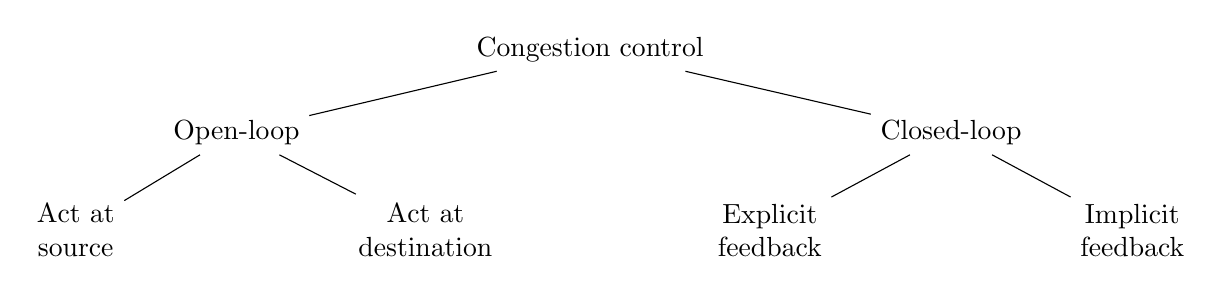
\begin{tikzpicture}
  \label{page:cc:cc_types}

  \node (cc) {Congestion control};
  \node [below left=0.5cm and 2cm of cc] (ol) {Open-loop};
  \node [below right=0.5cm and 2cm of cc] (cl) {Closed-loop};
  
  \node [below left=0.5cm and 0.5cm of ol, align=center] (src) {Act at\\source};
  \node [below right=0.5cm and 0.5cm of ol, align=center] (dest) {Act at\\destination};

  \node [below left=0.5cm and 0.5cm of cl, align=center] (expl) {Explicit\\feedback};
  \node [below right=0.5cm and 0.5cm  of cl, align=center] (impl) {Implicit\\feedback};

  
  \draw (cc) -- (ol) edge (src)-- (dest); 
  \draw (cc) -- (cl) edge (expl)-- (impl); 
  
\end{tikzpicture}

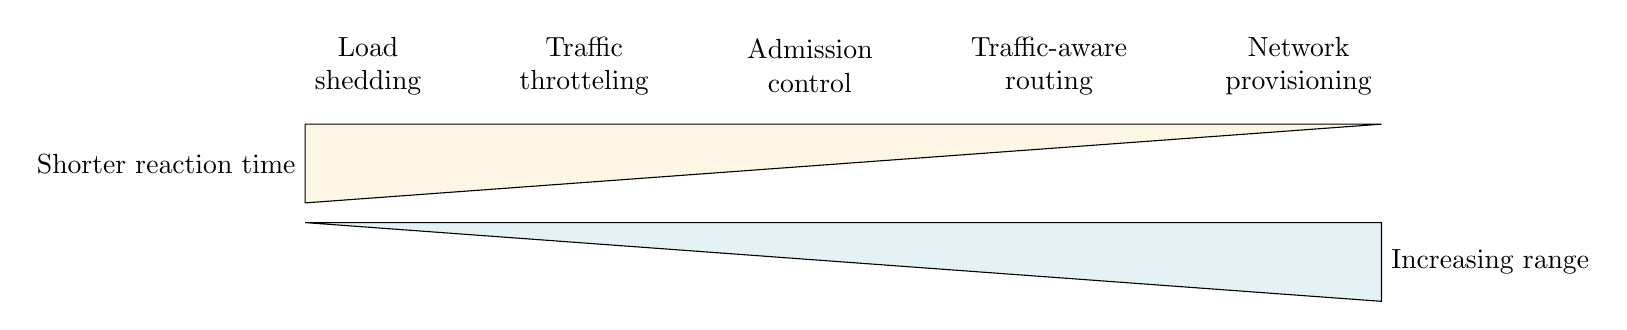
\begin{tikzpicture}[start chain]
  \label{page:cc:timescales}

    \begin{scope}[every node/.style={on chain, align=center}]
      \node (ls){Load\\shedding};
      \node{Traffic\\throtteling}; 
      \node{Admission\\control};
      \node{Traffic-aware\\routing}; 
      \node (np){Network\\provisioning}; 
    \end{scope}


    \draw [fill=hpiyellow!10] ([yshift=-0.25cm]ls.south west) to node[left] {Shorter reaction time} ++ (0,-1) -- ([yshift=-0.25cm]np.south east)  -- cycle; 

    \draw [fill=hpiblue!10] ([yshift=-1.5cm]ls.south west) -- ([yshift=-1.5cm]np.south east) to node[right] {Increasing range} ++ (0, -1) -- cycle; 
\end{tikzpicture}


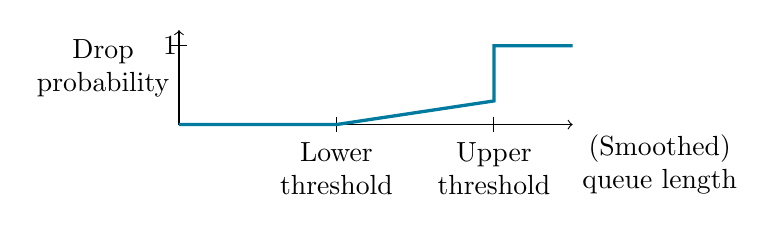
\begin{tikzpicture}[every node/.style={align=center}]
    \draw [->] (0,0) -- (0,1.2) node [below left, align=center] {Drop\\ probability};
  \draw [->] (0,0)  -- (5,0) node[below right, align=center] {(Smoothed)\\ queue length};
  \draw (-0.1,1) -- (0.1,1) node [left] {1}; 

  \draw (2, 0.1) -- (2, -0.1) node [below] {Lower\\threshold}; 
  \draw (4, 0.1) -- (4, -0.1) node [below] {Upper\\threshold};
  
  \draw [hpiblue, very thick] (0,0) -- (2,0) -- (4, 0.3) -- (4,1) -- (5,1); 
  
\end{tikzpicture}

\begin{tikzpicture}
  \label{page:cc:sawtooth}
  \draw [->] (0,0) -- (0,10) node [below left, align=center] {\Huge CWND};
  \draw [->] (0,0)  -- (20,0) node[below right, align=center] {\Huge Time/RTT};

  \draw [very thick]  (0,2) -- ++ (5,5) -- ++ (0,-3.5)  -- ++(4.5, 4.5) --  ++ (0, -4) -- ++(6,6) --++(0, -5) --++(3,3) -- ++(0,-4);
  
  
\end{tikzpicture}
\end{document}